%************************************************
\chapter{Methodology}\label{ch:methodology}
%************************************************

The purpose of this chapter is to first formulate the research questions that we examine in our work
and then propose our method of answering them.

\section{Research Questions}\label{sec:research_questions}

In the \nameref{ch:example_chapter} chapter we dicussed the different meanings of structural and dataflow-based interactions.
With this knowledge, we can answer many interesting research topics. 
These topics include patterns in feature development and usage of commits therin as well as findings about how likely seemingly unrelated commits are to affect features inside a program.

\subsection*{\textbf{RQ1: How do commits and features structurally interact with each other?}}

We intend to research two main properties which already provide a lot of insight into the development process of features and best practices of commits therein.

\subsubsection*{Investigating Patterns around Feature Development}

Firstly, we examine the number of commits features interact with structurally. 
This gives us a direct estimate on how many commits were used in the development of a feature.
Our analysis also allows us to measure the size of feature, which can put the number of commits used to implement a feature into perspective.
We refine our investigation by factoring in the nesting degrees~\ref{sec:nesting_degree} of our collected structural CFIs.
This allows us to additionally determine the \textsf{definite} size of a feature showing us to what extent its code is nested inside other features.
Furthermore, we can differentiate between commits that most likely and those that only potentially implement a feature's functionality.
By doing so, we intend to achieve a more accurate analysis regarding the number of commits used during a feature's development.

\subsubsection*{Examining the Usage of Commits in Feature Development}

Secondly, we investigate the number of features a commit usually changes by examining its structural CFIs. 
This is especially interesting when considering best practices surrounding the usage of commits.
It is preferred to keep commits atomic\cite{hundhausen2021commit_metrics} meaning they should only have a single responsibility.
As different features implement separate functionalities, it's unlikely for a commit to change several features while dealing with the same issue.
Transferring this to our work, high quality commits should mostly change a single feature.
Acquiring data on this issue might show how strictly this policy is enforced in the development of features across different projects. 
In section \ref{sec:commit_concerns}, we discussed that, due to feature nesting, a commit can structurally interact with multiple features at the same time while only changing functionality of one of them.
Instead of considering the features a commit structurally interacts, we rather examine the number of its feature-related concerncs~\ref{def:commit_concerns} for this RQ.
This way we aim to achieve a more accurate preditction for the number of features a commit changed or implemented.
In our analysis, we should ideally filter commits whose purpose was refactoring code, since they do not fit our criteria of changing or adding functionality to a feature.
Exceptionally large commits might be best considered for this, as this is where we expect most commits used for large-scale refactoring to appear.
A qualitative review of these commits is still necessary to make a final decision on whether they should be filtered.

\subsection*{\textbf{RQ2: How do commits interact with features through dataflow?}}

Investigating dataflow inside a program can unveil interactions between its entities that were previously hidden from programmers.
This can help them understand the extent to which different parts of a program influence each other.
Furthermore, deploying the introduced analysis in a direct manner could ensure improvements in the daily life of a developer.
In the context of our work, an example for this could be the faciliation of finding the cause of and subsequently fixing bugs in features.
Bugs occuring in certain features could be traced back to the commits responsible for them by factoring in recent commits affecting said features through dataflow. \\
Previous studies have laid the groundwork for researching dataflow interactions between different abstract entities of a program.
While it has shown a wide range of interesting use-cases, it has focused solely on dataflow between commits.
That's why we aim to provide first insights into the properties of dataflow-based CFIs.

\subsubsection*{The Proportion and Dependencies of Commits Affecting Features through Dataflow}

Firstly, we investigate how connected commits and features are by analyzing the number of features a commit affects through dataflow.
Knowing what fraction of all commits contributing code to a project are part of dataflow-based interactions can show how often new commits affect the data of a feature. 
Regarding this, it is worth considering the dependency dicussed in section \ref{sec:combination_cfis}, that structural interactions heavily coincide with dataflow interactions.
This implies that commits constituting code of a feature are very likely to influence said feature through dataflow as well.
In section \ref{sec:combination_cfis}, we also mention that the dataflow of commits not structurally interacting with a feature, must stem from outside the regions of the feature. 
Naturally, said dataflow is less intentional and subsequently more interesting, than dataflow occuring inside the regions of a feature. 
Programmers are less aware that changes introduced with these commits might affect the data of seemingly unrelated features.
Therefore, we intend to differentiate between dataflow interactions with an outside and those with an inside origin in our anaylsis.
This allows us to especially focus on commits part of outside dataflow interactions and examine their proportion among all commits. 

\subsubsection*{Understanding Features and the Commits Affecting them Through Dataflow}

Dataflow-based CFIs allow us to examine another interesting property, namely the number of commits affecting a feature through dataflow.
Here, we differentiate between commits \textsc{inside} and \textsc{outside} of features, i.e. commits that either do or don't contribute code to them.
We examine the proportion of outside to inside commits influencing a feature to gauge where most dataflow interactions of a feature stem from.
Considering our previous assumptions, the ratio of outside to inside commits could decrease with increasing size of a feature.
Smaller features are likely to structurally interact with less commits than their larger counterparts, resulting in them also interacting with less inside commits through dataflow.
However, the number of outside commits affecting data of a feature is not dependent on feature size in such a way.
This leads us to another relationship worth investigating, namely the relation between the size of a feature and the number of outside and inside commits interacting with it through dataflow.
We examine the two commit kinds separately, as we already have a strong supposition for inside commits, but are less certain for outside commits. 
Determining to what extent feature size is the driving factor in this relation, could tell us whether it is worth considering other possible properties of features in future analyses.

\subsection*{\textbf{RQ3: How do authors interact with features?}}

A simple yet promising way to extract more information out of the collected CFIs is to link the interaction's commits to their respective authors.
Thus, we are able to investigate how authors interact with features both structurally and through dataflow.
Similarly to the number of commits implementing a feature, we can now calculate the number of authors that participated in its development.
The same applies to commits interacting with features through dataflow, for which we can now determine the authors contributing these commits.
Here, we only consider outside commits, i.e. commits not constituting code of the feature, since we have already considered all inside commits when investigating the developers implementing a feature.
We are especially interested in how many authors exclusively interact with a feature through dataflow in comparison to the number of its developers.
This lets us determine whether the developers that implement features are also the ones mainly responsible for changes affecting them through dataflow. \\
Finally, we relate both types of author interactions to the respective size of a feature.
Regarding structural interactions, this allows us to determine whether a feature's extent in the source-code of a project is driving factor in the amount of authors needed to implement it. 
Software companies could use evidence on this issue as advice on how to allocate programmers on to-be implemented features.
Findings on the investigated dataflow interactions of authors could tell developers that their changes might affect small and, at first sight neglegible, features surprisingly often.
We also have a look at the specific functionality of features since their purpose could also play an important role in the number of authors interacting with them.

\begin{center}
\begin{tabular}{cc}
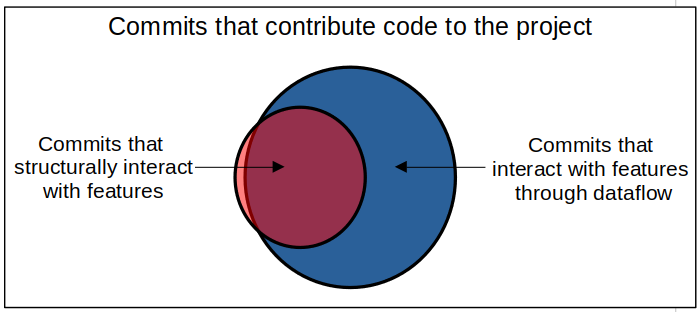
\includegraphics[height=6cm]{gfx/Commits-of-a-Software-Project.png}
\end{tabular}
\captionof{figure}{Illustration of different commit kinds}
\end{center}
\textsf{
In the first two \textbf{RQs} we have discussed different kinds of commits and the ways in which they interact with features. 
The above figure showcases them in a venn diagram and illustrates the dependencies and divisions between them.
}

\section{Operationalization}\label{sec:operationalization}

Here, we explain how the proposed RQs can be answered.
The general experiment process is the same for all RQs.
At first, we collect data comprimising all structural or dataflow-based CFIs by creating reports of a specific type for a chosen software project.
The collected data is then processed in order to gain information for each commit or feature in the project, such as the number of interacting commits and size of a feature.
The processed data is used to calculate statistical information, such as the mean and variance, or the strength of a correlation.
To facilitate a faster and better understanding of the processed data and calculated statistics, we display them graphically via bar or regression plots.
The projects we investigate in this work, for example \textsc{xz} and \textsc{gzip}, are of a small size and are used in a compression domain.
This choice is based on the fact, that our research intends to only lay basic groundwork, where smaller projects can already offer a lot of insight.
Since we only investigate a few projects, we chose them to be of a similar domain, such that a comparison between them makes more sense.
In the following sections, we explain our method of investigation in more detail for each RQ.

\subsection*{\textbf{RQ1: How do commits and features structurally interact with each other?}}

For this RQ, we examine the interactions contained in the structural reports created with our implementation in VaRA.
As there could be vast differences between the projects, we also work with and present their respective data separately.

\subsubsection*{Investigating Patterns around Feature Development}

From the collected structural reports, we first extract the number of structurally interacting commits and size for each feature.
For each interacting commit, we also determine the nesting degree of its structural interaction with the feature.
Additionally to the normal size of a feature\ref{sec:feature_size}, which we call \textsf{potential} size, we calculate its \textsf{definite} size as well. 
The datapoints of the two properties are shown in two respective bar plots, where the values for each feature are shown in a separate bar.
The bars are labelled after the name of the feature they present, to allow for comparisons between the two plots and between different projects.
For comparisons between the investigated projects, we also calculate the average number of interacting commits and size of a feature for each project.
In the plot displaying the number of interacting commits, we stack the commits according to the nesting degree of their respective interaction with the feature.
The first part of each bar consists of commits interacting at a nesting degree of one, the second part of commits interacting at a higher nesting degree.
We do the same in the second plot, where the definite size forms the base of each bar upon which the difference with the potential size is added.
This also allows us to see how common feature nesting is inside a project and which features are nested inside other features.
Logically, the stacked bars must be colored differently to see their respective distribution inside a feature.
The y-axis represents the number of instructions implementing a feature, i.e. the number of instructions stemming from its feature regions.
The definite size of a feature only consists of instructions that are exclusively part of its respective regions, whereas we also count instructions part of multiple regions for the potential size of a feature.
The features are sorted in an increasing order according to total the number of interacting commits interacting or size.
Finally, we relate the two investigated properties in a \textsc{seaborn} regression plot.
Here, we show whether features increasing in size, in turn structurally interact with more commits, i.e. need more commits to be implemented.
Therefore, the value of the x-axis shows the size of a feature, whereas the y-axis shows the number of interacting commits.
Each feature is represented by a scatter point inside the plot combining its respective y-values from the two previous plots.
A linear regression line is drawn in the plot matching the occuring scatter points, where a rising graph could already indicate a positive correlation.
To check whether we are dealing with a statistically significant linear correlation, we compute the pearson correlation coefficient and its p-value in the \textsc{stats} submodule of the \textsc{scipy} python namespace.
To confirm our initial suspection of a strong positive correlation, the according correlation coefficient must be close to one, while the p-value must be close to zero falling below our rejection interval of 95\%.
Here, we only consider the total number of interacting commits and size of a feature, which are the entire bar-values of a feature.
To underline this, we choose the color of the regression plot as a mixture of the two colors used in the bar-plots.

\subsubsection*{Examining the Usage of Commits in Feature Development}

For each commit part of at least one structural interaction, we determine the number of its concerns~\ref{def:commit_concerns}.
For this, we examine the complex structural CFIs discussed in our \nameref{ch:implementation}.
There, we increment the number of a commit's concerns upon finding a new set of features it structurally interacts with at the same time, i.e. within the same instructions.
Following this, we give a comprehensive overview of our results in a \textsc{seaborn} histplot for every investigated project.
The x-axis of the histogram shows the number of a commit's concerns, whereas the y-axis shows the number of commis for which the respective x-value matches.
If 50 commits deal with a single concern inside a project, the y-value of one will be 50 accordingly.
Thus, we can quickly see to what extent our derived best practice surrounding commits in feature development is enforced in a project.
The more commits are located at one in comparison to other x-values, the more commits are likely to have only changed a single feature.
To facilitate comparisons between projects, we choose the same x- and y-labels for every histogram. 
Commits with exceptionally many concerns are shown in an additional x-tick to avoid an overly long x-axis.
Instead, we mention these commits explicitly during our evaluation and relate the number of their concerns to their specific purpose. \\
In a second analysis step, we filter exceptionally large commits, whose purpose we expect to be something else than implementing features, such as code-refactoring.
Similiarly to the regions of a commit, we determine its size in a repository as the number of source-code lines that were last changed or added by it.
We then apply tukey's fence with a k-value of 3 to filter far outliers of commit sizes among commits interacting with features within their respective project.
Afterwards, we perform a qualitative review of the filtered commits to check whether our initial suspicion about their purpose is correct.
To asses the effect of filtering exceptionally large commits, we compute the average number of concerns within a project before and after the application of our restriction.
Both averages are subsequently shown in a cross-project table so that we can compare them within a project and recognize a general trend among them.

\subsection*{\textbf{RQ2: How do commits interact with features through dataflow?}}

The projects investigated for dataflow-based CFIs are the same projects as investigated for structural CFIs.
This choice gives us more insight into a single project and allows us to combine both analysis results as will be discussed below.

\subsubsection*{Analyzing the Proportion and Dependencies of Commits Affecting Features through Dataflow}

We do not consider \textsc{lrzip} here, as we are only able to detect regions of three out of 10 features in the project.
This means that we can only find a fraction of all commits interacting with features, resulting in significantly lower determined proportions. \\
An initial step of evaluating what fraction of commits affect features through dataflow, is determining which set of commits to consider in the first place.
Logically, we should only consider commits that could potentially be part of a dataflow-based CFI.
The only prerequesite for this is that commits are represented by commit regions inside a program.
This is the case when there exists at least one source-code line that was last changed or added by them.
We call the respective commits, \textsf{active} commits as their contributed code is still ``active'' in the repository.
Following the calculation of the number of active commits in the projects, we begin examining the created dataflow reports.
For each commit part of at least one dataflow-based CFI, we save the set of features it interacts with.
By dividing the number of these commits by the number of all active commits, we can determine their proportion within their respective project.
To allow for an overview of all projects, we show the calculated percentages in a \textsf{seaborn} bar plot.
To provide evidence for our claim that structural CFIs heavily coincide with dataflow-based CFIs, we now compute the proportion of commits with dataflow interactions among the commits with structural interactions.
Given that the latter is significantly higher than the overall proportion of commits with dataflow interactions, our initial notion will be confirmed.
Alongside the percentage of commits part of dataflow-based CFIs, we also show the percentage of active commits that are part of structural CFIs.
As we expect most of the latter commits to be part of dataflow-based CFIs as well, the difference between their respective percentages indicates what proportion of commits interact with features exclusively through dataflow.
The percentage of commits with dataflow interactions is certainly higher than the percentage of commits with structural commits, as the latter commits largely contribute to the former, while this does not need to be the case vice versa.
Following the broad overview of commits affecting features through dataflow, we intend to specify and differentiate between the origin of said dataflow.
For each feature a commit interacts with through dataflow, we check whether they also structurally interact with each other.
If they do structurally interact, we speak of an inside dataflow origin, otherwise we speak of an outside origin.
Afterwards we can split the commits with dataflow interactions into three categories.
Next to commits that only affect features either through inside or through outside dataflow, a commit can also interact with multiple features, once through inside and once through outside dataflow.
For each project, we calculate the respective percentages of each category and present them in a stacked bar plot.
Logically, each bar representing a project adds up to 100\% as every commit falls into exactly one category.
The commits falling into categories of at least partial outside dataflow origins are part of interactions, which we could only detect with our dataflow analysis.
Both bar plots are displayed next to each other in the same figure, where the sequence in which the projects are shown in both plots is determined by the proportion of commits with dataflow interactions.
This allows for an easier comparison within a project, as its respective bars will have the same position in both plots.
Statistical values, including the number of active commits and the probability for a commit to be part of a dataflow-based CFI given that it structurally interacts with features, are not included in the plots.
As they can aid the understanding of the plots and add important context to them, we display the respective values in a \textsc{latex} table.

\subsubsection*{Exploring Features and the Commits Affecting them Through Dataflow}

Intially, we determine the set of commits each feature interacts with through dataflow.
The according information is extracted from the same dataflow reports used in the previous section of this RQ.
Depending on whether the commit also structurally interacts with a feature, we split the set of commits for each feature into two categories.
Outside commits are fully located outside the regions of a feature, meaning that their data flows into a feature.
Inside commits are at least partially located inside a feature making it very likely that their dataflow occurs within the regions of a feature.
Naturally, said dataflow affecting a feature is less interesting than dataflow stemming from seemingly unrelated commits.
To gauge what commit kind makes up the majority of commits affecting features through dataflow, we present both values for each feature in a \textsc{seaborn} bar-plot.
For every examined project, we display the number of outside and inside commits with separate bars for the different features.
To enable an exact comparison, we also calculate the median for both outside and inside commits of a project.
We choose the median and not the mean, as we are especially interested in detecting a general trend across the features of a project and intend to avoid outliers skewing the data in one direction.
Besides that, features with an exceptionally high number of interacting commits or a high proportion of commits of a certain kind are already shown in the bar plots.
The features are explicitly named to allow for cross-project comparisons of certain types.
In a second analysis step, we now relate the size of a feature to the number of commits affecting it through dataflow.
Here, we are interested in determining whether and to what extent there exists a positive linear relationship between the two.
We employ two linear regression analyses, relating the size of a feature once to its outside and once to its inside commits.
Similarly to our investigation in \textbf{RQ1}, the results are displayed in a \textsc{seaborn} reg plot for each project.
In each regression plot, we also show the two computed pearson correlation coefficients and their respective p-values.
We decide for a 97.5\% rejection interval again, meaning that the p-values must be lower than 0.025 to provide enough evidence that the two datasets are indeed not un-correlated.
Furthermore, the correlation coefficient must range close to 1 in order to warrant a strong positive correlation.
Lastly, we investigate our claim that smaller features have a higher proportion of outside to inside commits affecting it through dataflow.
For this, we examine the relation between the size of a feature and the ratio of its outside to inside commits.
Again, we create linear regression plots for each project and calculate the acccording pearson correlation coefficients and the respective p-values.
We could also perform other regression analyses, for example a logarithmic regression, as they could fit our datapoints better.
Following our explanations in section \ref{sec:research_questions}, we expect the ratio of outside to inside commits to decrease with increasing feature size.
This would result in a negative linear correlation coefficient and a falling linear regression line.
It remains to be seen whether the respective values are statistically significant across several projects.

\subsection*{\textbf{RQ3: How do authors interact with features?}}

Technically, we perform the same analysis regarding features as discussed for the two previous RQs.
The only difference is that we replace the commits interacting with a feature with their respective authors.
To faciliate expressing this, we simply say that the respective authors interact with features based on a certain interaction type or that they are a feature's structural or dataflow authors.
In section \ref{sec:research_questions}, we mentioned that we only consider commits outside of features when examining the authors interacting with them through dataflow.
The computation of these commits has already been explained in the operationalization of RQ2, which we reuse for this RQ.
The number of authors that interact with a feature either structurally or through dataflow are presented in a \textsc{seaborn} bar plot.
Similarly to the previous RQs, the results of each project are shown in separate plots with labeled ticks for each feature.
We also calculate the mean number of dataflow and structural authors of a project to give concrete information from what type of interaction most author interactions stem from.
In a third bar for each feature, we display the number of authors that exclusively interact with them through dataflow.
There, we exclude authors who also structurally interact with the feature, i.e. the authors making up the first bar.
This shows us how many authors affecting a feature can only be determined via our dataflow analysis.
For the structural interactions of authors, we compute what fraction of them also affect the respective features through dataflow.
This can tell us to what extent the developers implementing a feature are likely to introduce code changes whose data the feature uses later on.
Additionally considering whether there are more structural than dataflow authors lets us determine whether the developers of a feature are also the ones mainly responsible for changes affecting them through dataflow.
Finally, we perform the same linear regression anaylsis as we have done for feature-sizes and the number of commits that interacting with them.
By calculating the strength of their correlation, we are able to determine whether the presumed extent of a feature inside a project is an accurate predictor for the number of developers needed to implement it.
The authors interacting with a feature through outside dataflow are also indirectly involved in its development, since the data stemming from their contributed commits is necessary for the functionality of the feature.
